\section{Resultados}

En este apartado se realizará una explicación en profundidad de las pruebas que se han realizado
para validar y verificar la implementación descrita en apartados anteriores. Esta sección
describirá desde el \textit{dataset} utilizado para la experimentación, hasta la ejecución
de las distintas pruebas lanzadas con diferentes configuraciones y variantes de nuestro 
algoritmo, mostrando en detalle los resulados obtenidos y su análisis. Además, se dará respuesta
a las preguntas de investigación planteadas en la Sección \ref{sec:research_questions}, lo que
constituye el objetivo principal de este estudio.


\subsection{Descripción del \textit{dataset} para experimentación}
Para realizar la experimentación, se han utilizado $20$ proyectos de código abierto disponibles
de forma pública en \textit{GitHub}. Todos los proyectos están basados en \textit{Java} y
han sido seleccionados de forma manual. Con el objetivo de tener una experimentación diversa,
se han tenido en cuenta dos escenarios posibles:

\begin{enumerate}
    \item \textbf{Escenario $1$}: engloba a todos aquellos proyectos donde la  CI falla con muy
    poca frecuencia. En nuestra solución, se ha considerado a todos estos proyectos como
    ``proyectos difíciles'', y serán todos aquellos en los que la proporción de \textit{build
    failures} es inferior al $10\%$ con respecto a las \textit{builds} exitosas.\\

    \item \textbf{Escenario $2$}: engloba a todos aquellos proyectos donde la CI falla con
    una frecuencia ``normal''. Consideramos como ``proyectos normales'' a todos aquellos en los
    que el porcentaje de \textit{build failures} se encuentra comprendido entre el $10\%$ y el
    $25\%$ con respecto a las \textit{builds} exitosas.\\
\end{enumerate}

Al incluir tanto proyectos difíciles como normales, se pretende obtener una visión más amplia
de la efectividad de nuestro algoritmo en diferentes condiciones y escenarios. Este enfoque
es beneficioso por varias razones:

\begin{itemize}
    \item \textbf{Evaluación en escenarios específicos}: separar ambos escenarios nos permite
    analizar el comportamiento del modelo en cada tipo de proyecto de forma más precisa.\\

    \item \textbf{Fortalezas y debilidades}: al evaluar cada conjunto de proyectos individualmente,
    podemos identificar fortalezas y debilidades del modelo en cada escenario.\\

    \item \textbf{Adaptabilidad del modelo}: al evaluar el modelo en diferentes escenarios, podemos
    observar si el modelo es capaz de adaptarse bien a ambos tipos de proyectos, o si realmente
    necesita un enfoque diferente para cada uno de ellos.\\
\end{itemize}

Se ha decidido catalogarlos como ``proyectos difíciles'' y ``proyectos normales'' según la
capacidad que tendrá el algoritmo de aprender de los \textit{build failures} en cada tipo de 
proyecto. En los proyectos difíciles, donde se espera que la proporción de \textit{build
failures} sea mucho menor a la de \textit{builds} exitosas, el algoritmo tendrá que aprender
de un número mucho menor de ejemplos de fallos, haciéndole la tarea de aprendizaje más difícil.
Por otro lado, en los proyectos normales, donde la proporción de \textit{build failures} es
más alta, el algoritmo tendrá más ejemplos de \textit{build failures} sobre los que aprender,
esperando que la capacidad de aprendizaje sea mayor.\\

Como hemos mencionado anteriormente, se han seleccionado $20$ proyectos de código abierto
disponibles en \textit{GitHub}. Cada uno de ellos ha sido seleccionado de forma manual, y se
ha intentado que el número de \textit{builds} sea lo más similar posible entre ellos. A
continuación, se muestran dos gráficos que describen la proporción de \textit{build failures}
en cada uno de los proyectos seleccionados, tanto para proyectos difíciles como para proyectos
normales.\\

\begin{figure}[H]
    \centering
    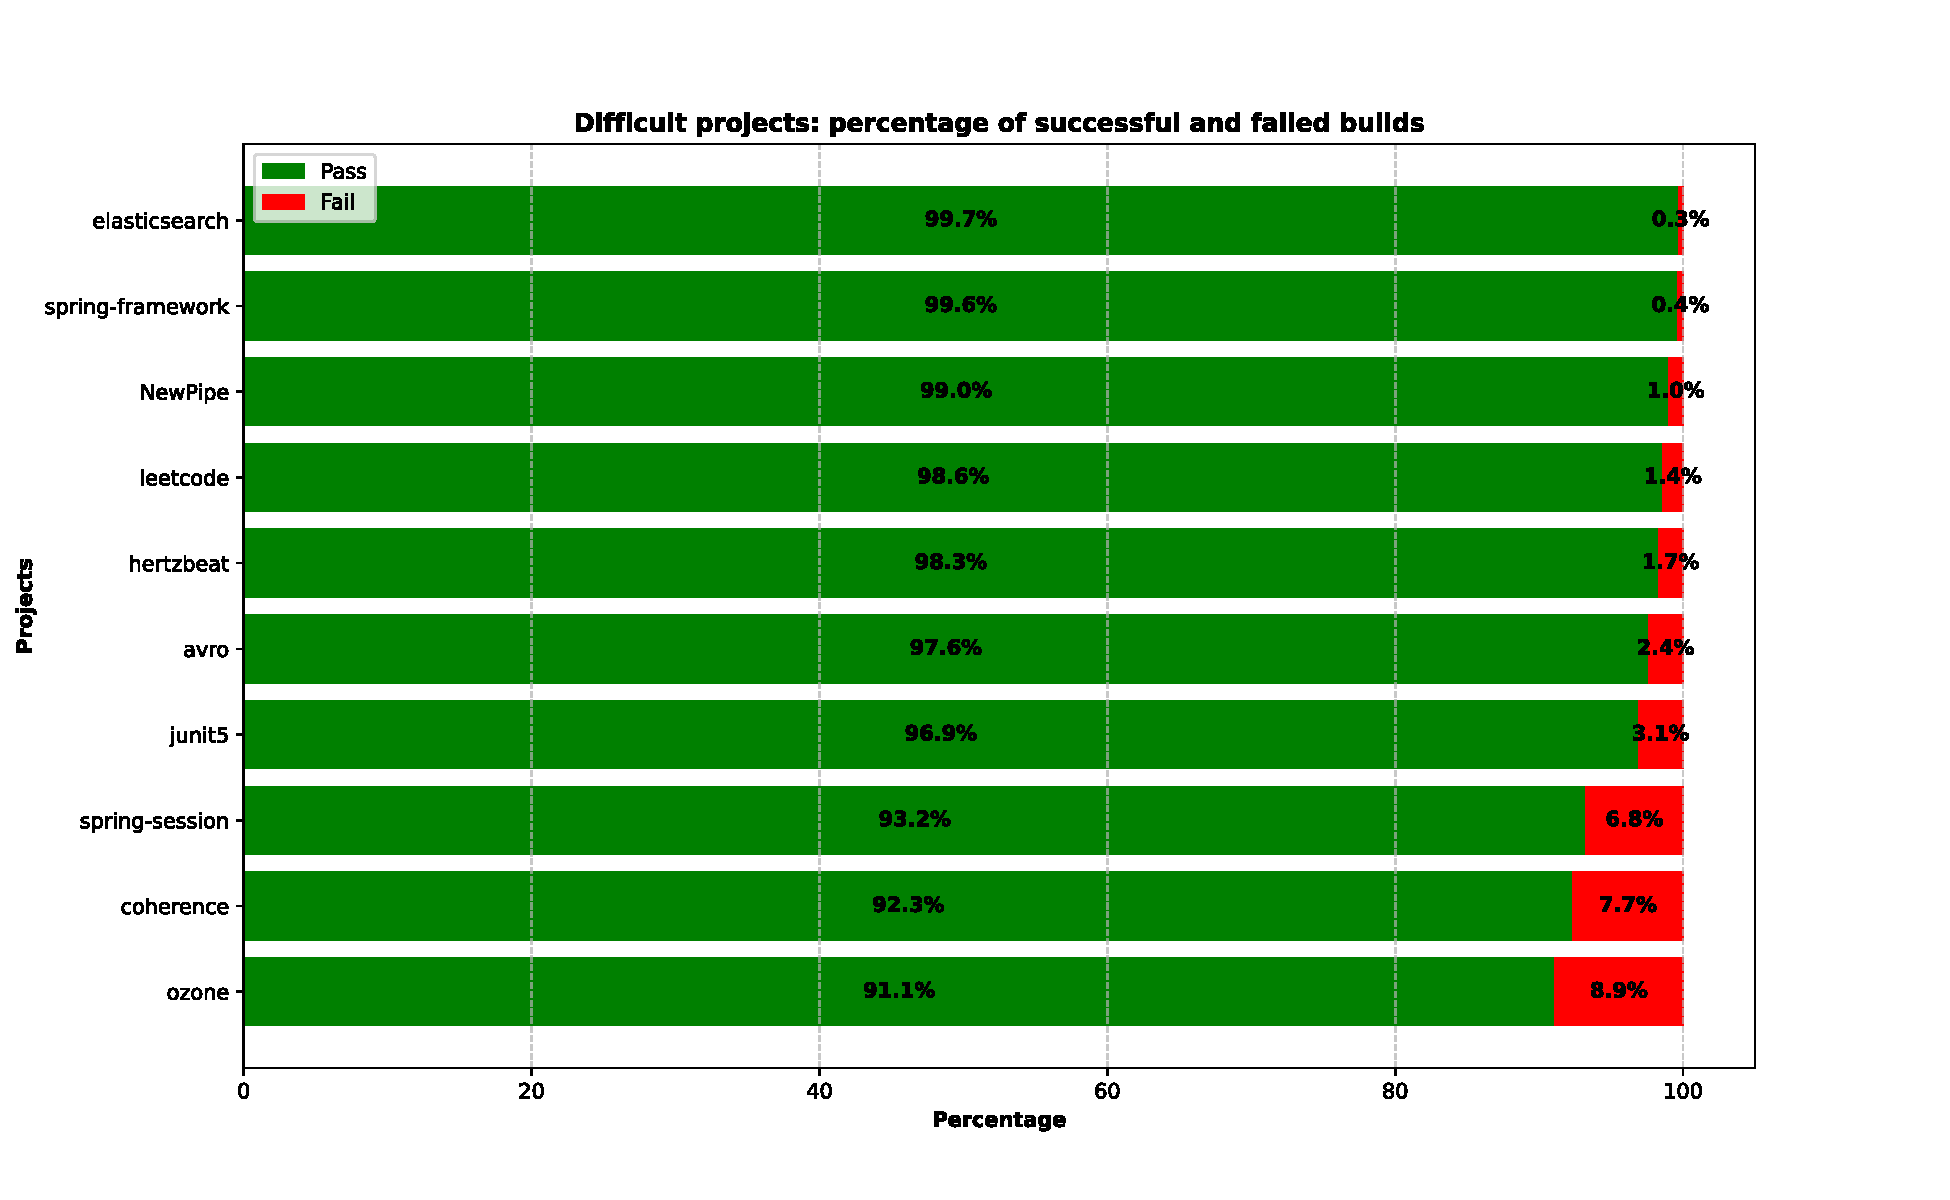
\includegraphics[width=0.85\textwidth]{images/Failures_difficult_projects.pdf}
    \caption{Proporción de \textit{build failures} en proyectos difíciles}
    \label{fig:failures_difficult_projects}
\end{figure}

\begin{figure}[H]
    \centering
    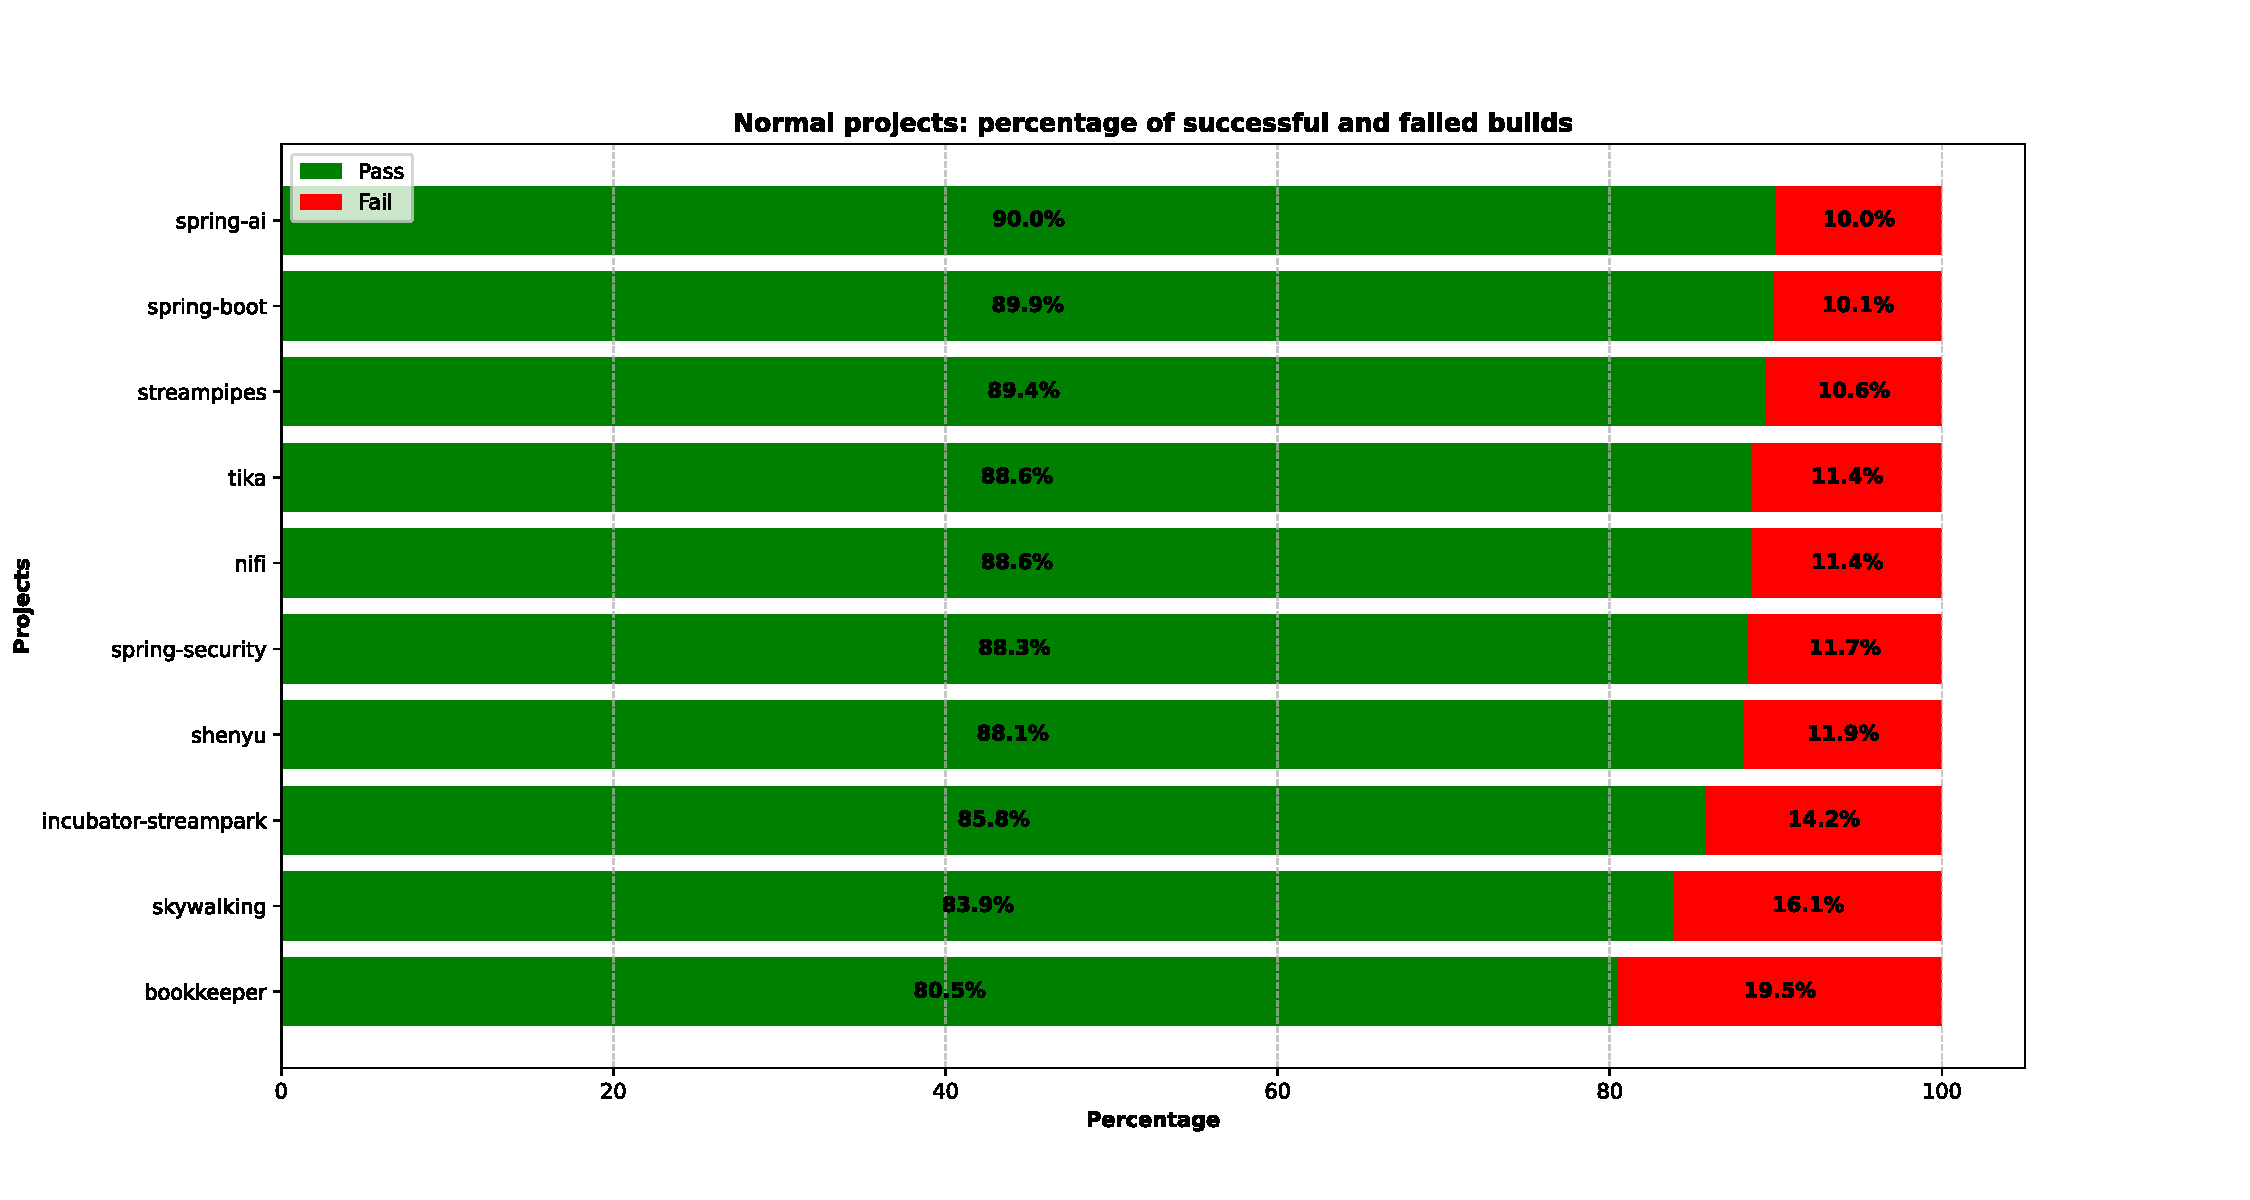
\includegraphics[width=0.85\textwidth]{images/Failures_normal_projects.pdf}
    \caption{Proporción de \textit{build failures} en proyectos normales}
    \label{fig:failures_normal_projects}
\end{figure}

Como vemos, en los proyectos difíciles la proporción de \textit{build failures} es inferior al
$10\%$, mientras que en los proyectos normales se encuentra entre el $10\%$ y el $25\%$. En
ambos casos, se ha intentado que el número de \textit{builds} sea lo más similar posible entre
los proyectos seleccionados.\\


\subsection{Descripción de pruebas y análisis de resultados}
